\section{The Microconnectome}
Here we introduce the Bio-M MC. This is one of the microcircuits that the BBP reconstructed. It represents the mean measurements of a set of 5 other varying instantiations of a rat's neocortical column.
\subsection{Bio-M MC}
\subsubsection{Origins of the Bio-M MC}
The Blue Brain Project have created multiple variants of a rat's neocortical column (a microconnectome). These are  comprised of 6 sets of 7 statistically varying instantiations. The first 5 of these sets were based on specific heights of the layers in the neocortex. These instantiations ultimately gave rise to a set of average instantiations of the neocortical column. The instance that focus on here is the final instance in this set of averages, the Bio-M MC. This instance of the neocortical column contains 6 layers, that are made up from a total of 55 different morphological neuron types. These can be further differentiated into excitatory and inhibitory neurons. The Bio-M MC representing the circuit itself contains approximately 7.8 million synaptic connections represented as directed edges that connect the 31,346 neurons represented as vertices. 

\begin{figure}[H]
\begin{center}
\captionsetup{justification=centering}
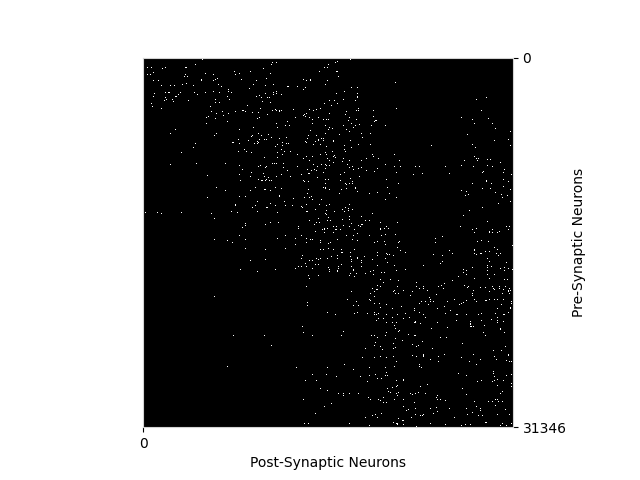
\includegraphics[width=12cm]{BioM/matrix_BioM.png}
\caption{Adjacency Matrix for the Bio-M MC}
\end{center}
\end{figure}
%----------------------
\subsubsection{Block Layout}
\begin{figure}[H]%
    \centering
    \captionsetup{justification=centering}
    \subfloat[\centering Block-wise Edge Densities]{{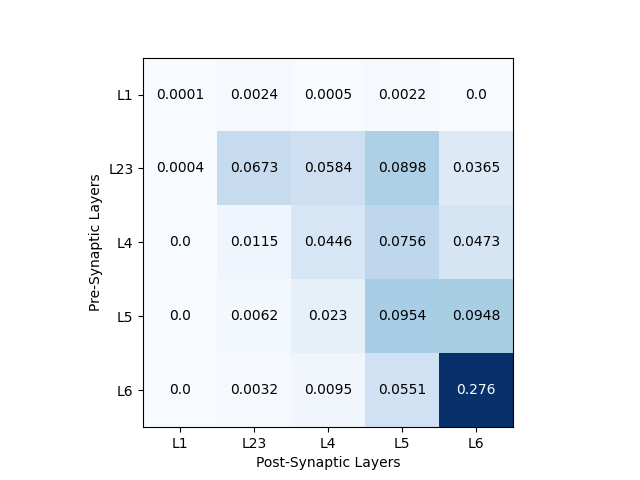
\includegraphics[width=7cm]{BioM/heat_map_layer_BioM_dens_sci.png} }}%
    \qquad
    \subfloat[\centering Block-wise Edge Counts]{{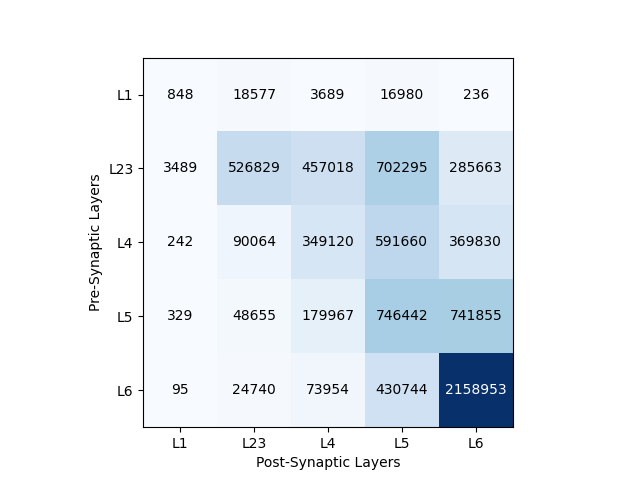
\includegraphics[width=7cm]{BioM/heat_map_layer_BioM.png} }}%
    \caption{Connectivity by block of the Bio-M MC}%
    \label{fig:example}%
\end{figure}

To help visualise the MC, in Figure 5, we have a graphical representation of the connectivity of the neurons as they pass from the pre-synaptic neuron to the post-synaptic neuron in the form of an adjacency matrix. The rows represent the pre-synaptic neurons and the columns represent the post-synaptic neurons. As can be seen here, there is a large number of these connections in the leading diagonal which represents the connections within the layers as compared to off-diagonal blocks that represent connections between the layers, as can be seen in Figure 6. Furthermore, we see that there is a large number of connections that are contained within layer 6. The number of connections in this block amounts to approximately 27\% of all connections in the Bio-M MC.

The volume of the Bio-M MC is approximately $0.29$mm$^3$. The relative thickness is shown in Figure 7, along with statistical details of each layer shown in Table 2.


\begin{center}
\begin{table}[H]
    \centering
    \captionsetup{justification=centering}
     \begin{tabular}{||c | c | c | c||} 
 \hline
 Layer & Thickness(\(\mu\)m) & Neurons & Density(neurons/mm\(^3\)) \\ [0.5ex] 
 \hline\hline
 1 & 149 & 339 & 14706 \\ 
 \hline
 2/3 & 502 & 7519 & 31466 \\
 \hline
 4 & 190 & 4661 & 51074 \\
 \hline
 5 & 525 & 6106 & 24214 \\
 \hline
 6 & 700 & 12722 & 37838 \\ 
 \hline
 \hline
\end{tabular}
    \caption{Statistical details of the Bio-M MC}
    \label{tab:my_label}
\end{table}

\end{center}
\begin{figure}[H]
\begin{center}
\captionsetup{justification=centering}
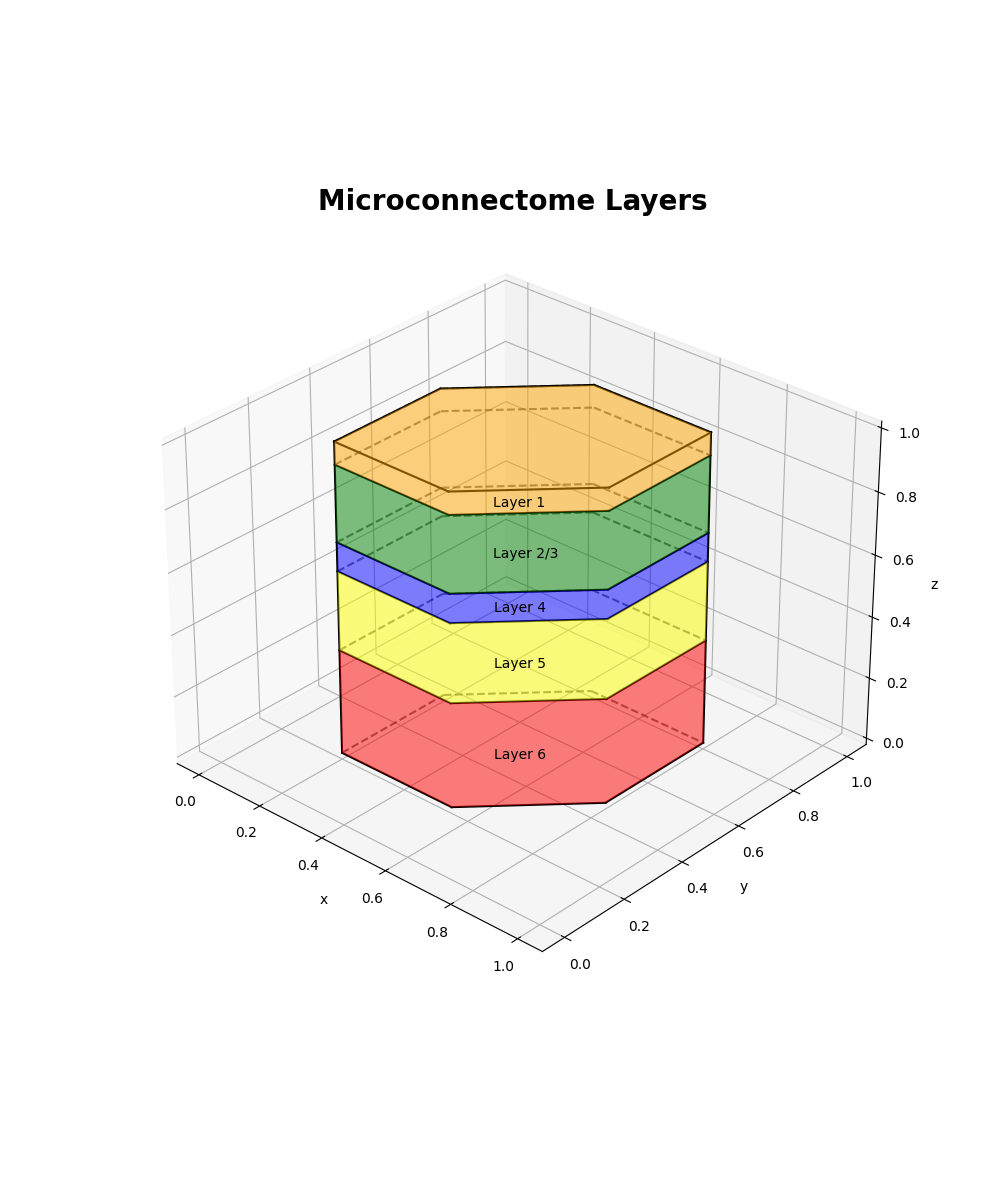
\includegraphics[width=10cm]{BioM/connectome.png}
\caption[center]{Neocortical column scaled to account for layer thickness}
\end{center}
\end{figure}



\subsubsection{Distance Distribution}
To see further how the models compare to the original structure of the Bio-M MC, we also want to take a look at distances between the connected neurons to see how much of an impact distance has on the level of connectivity within the MC. Since our models are only dealing with the neurons and the observed synaptic connections that are present in the Bio-M MC, we look only at the functional graph, as shown in Figure 8.

\begin{figure}[H]
\begin{center}
\captionsetup{justification=centering}
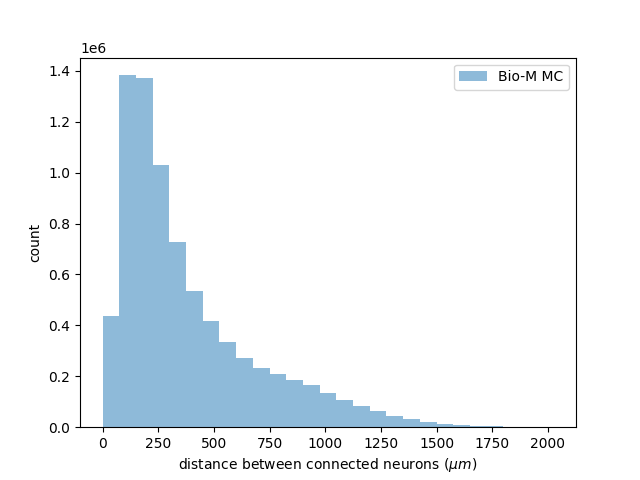
\includegraphics[width=10cm]{BioM/BioM_dist_distr.png}
\caption{Distance distribution of connected neurons in the Bio-M MC}
\end{center}
\end{figure}

We have taken the bin sizes to be 75\(\mu\)m, to be consistent with the distances that were proposed in \cite{Reimann_2017}. This is due to 75$\mu$m being the maximum bin size that preserved the distribution of soma-distances of connected neurons in all sub-matrices of the adjacency matrix representation of the MC. A sub-matrix here, is defined by the connections between a morphological neuron to another morphological neuron type. By example, we have L1 DAC to L1 HAC. This is just one example of the 3025 sub-matrices that are contained in the MC. More details of this are given in the section on the General Biological model.

\subsubsection{Signed Degree of Neurons}
In Figure 9, we have the signed degree of the neurons. These are calculated by taking the neurons in-degree minus the out-degree. Therefore, a positive value as shown in Figure 9(a), indicates that the information flow into the neuron is greater than the flow out and vice versa for a negative degree. So, from Figure 9(a), we can see that more flow is directed towards the neurons that are located in layers 1, 2 and 3 and that more flow moves away from the neurons in layers 4, 5 and 6. This, theoretically, is down to the fact that L4 is the major thalamorecipient layer and therefore a starting point of cortical information processing. Subsequently, information is then propagated through the cortical column, firstly to L2/3, then from there to L5 and L6, which are the primary output layers of the cortex \cite{10.3389/fnana.2017.00091}. 

To show that the graph representing the network is finite, we can take the sum of signed degree for each neuron over the set of neurons, $\sum_{v \in \mathcal{G}}\sd(\emph{v}) = 0 \enspace{.}$ Figure 9(b) shows the cumulative sum of the signed degree of each neuron throughout the MC. All models barring the \ER model follow this pattern as we aim to preserve this. 

\begin{figure}[H]%
    \centering
    \captionsetup{justification=centering}
    \subfloat[\centering Signed Degree of each neuron in Bio-M MC]{{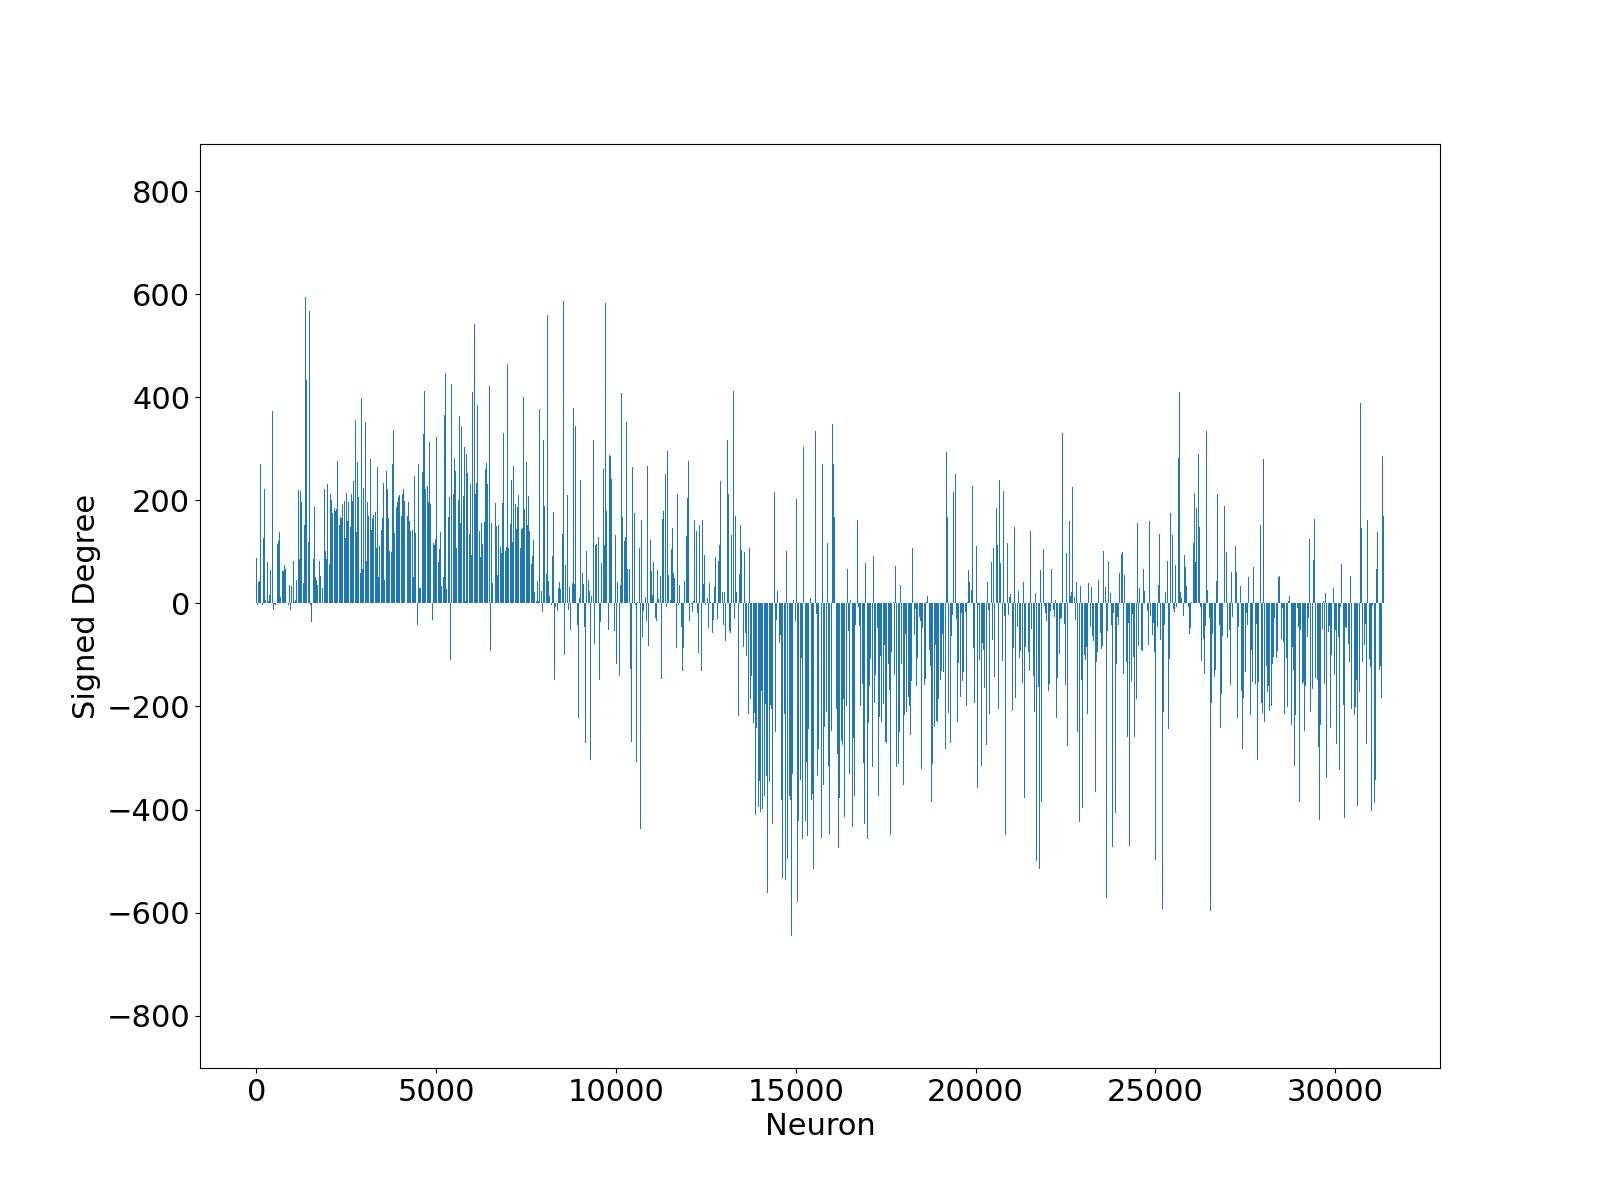
\includegraphics[width=7cm]{BioM/BioM_sd.png} }}%
    \qquad
    \subfloat[\centering Cumulative sum of signed degree to show graph $\mathcal{G}$ is finite]{{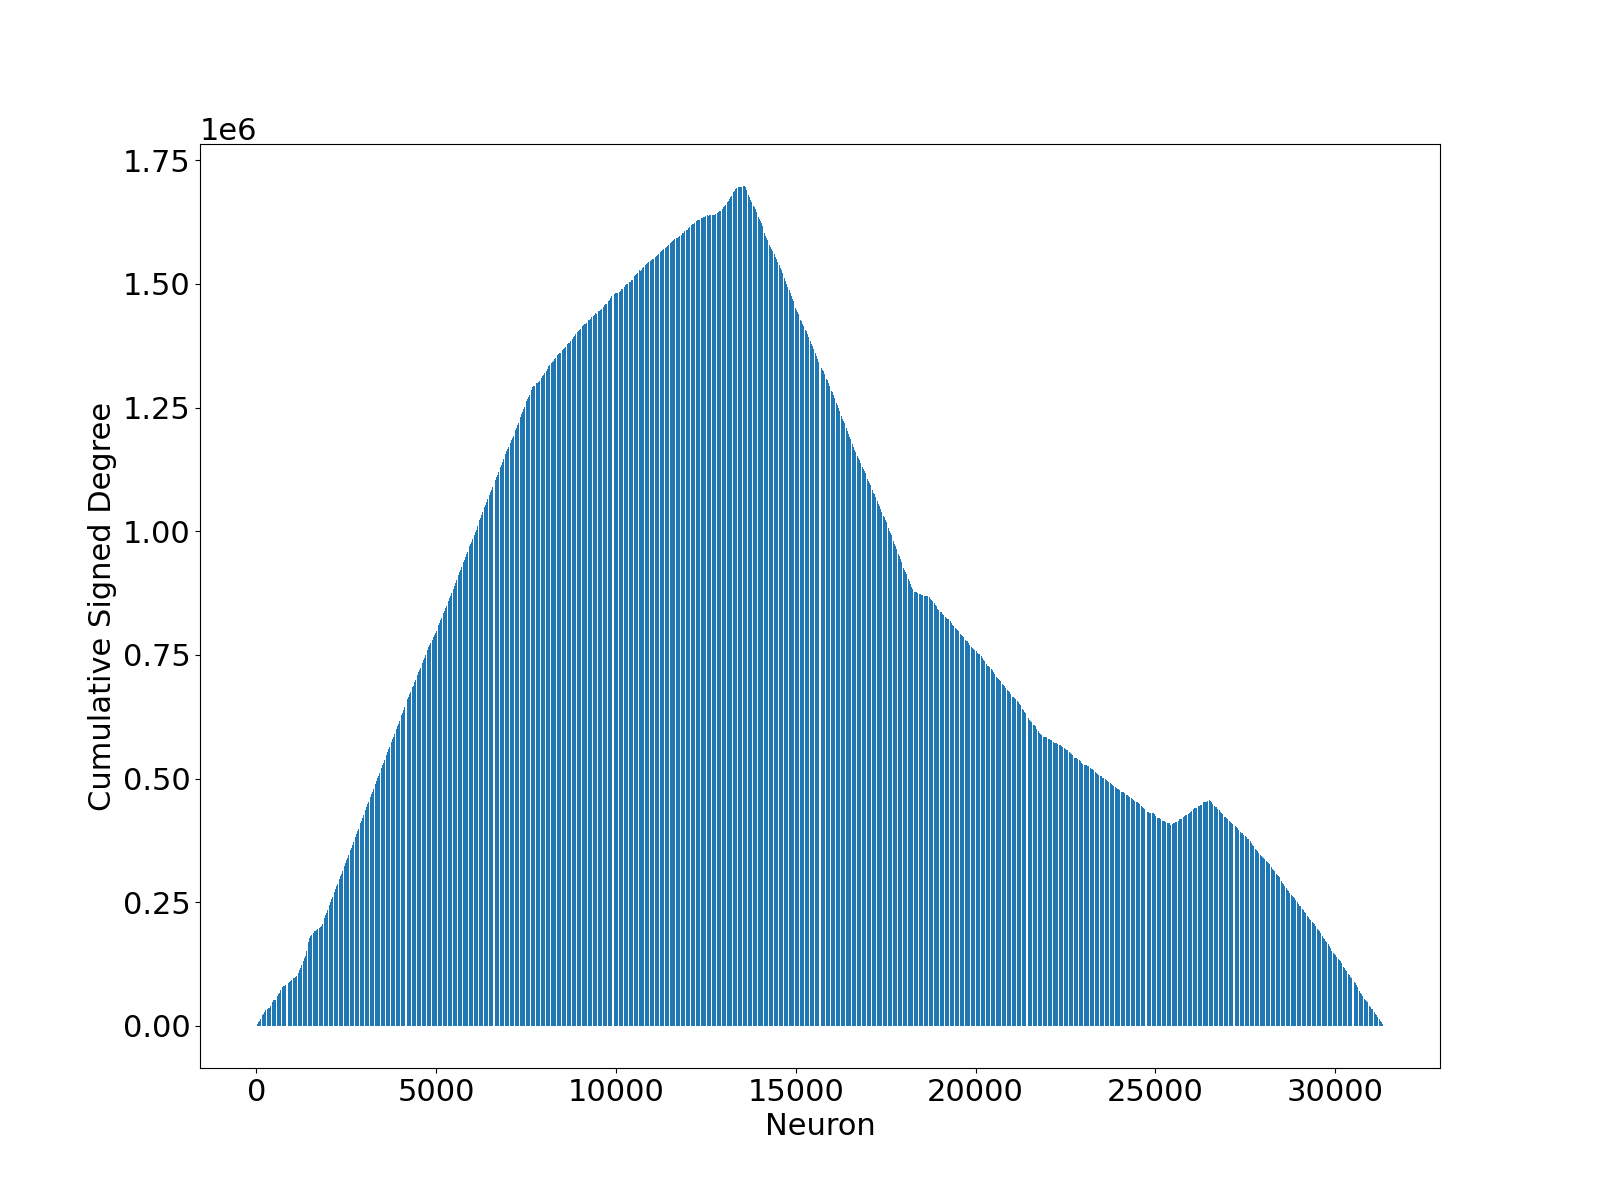
\includegraphics[width=7cm]{BioM/cumsum_degree_BioM.png} }}%
    \caption{Signed Degree statistics for the Bio-M MC}%
    \label{fig:example}%
\end{figure}